\chapter{Free Energy Calculations}

\section{Basics}

In the last few years, the accuracy and feasibility of free energy calculations
improved significantly \cite{King.2021}. The main reasons are developments
in the accuracy of force fields\cite{Cournia.2017}, the increase
in computational resources and, in particular, the usage of graphics
processing units to cope with the high computational demands. By now,
most MD software packages, like AMBER\cite{DavidA.Case.2005}, CHARMM\cite{Brooks.2009} or GROMACS\cite{Abraham.2015}, offer functions
for alchemical free energy calculations which facilitates the set-up
of such simulations. 

Possible applications can be found in rational drug design and drug
discovery; e.g., during lead optimization, the binding free energy differences
between compounds are of interest.\cite{Cournia.2017} As the free energy difference
 provides information about the thermodynamic favorability of a specific
process, it can help to find ligands that bind most tightly to a biomolecule of
interest.

One can distinguish between absolute and relative free energy calculations:
Absolute free energy differences are, for instance, solvation or binding
free energy differences of one compound (these results can be compared
with the free energy of an unrelated compound)\cite{Boresch.2003,Jorgensen.1988},
whereas the latter approach computes the free energy difference between,
e.g., two ligands, which usually are related to each other. For many
practical problems, such knowledge is sufficient, for instance, when
the comparison of properties like binding affinity of two ligands
is sought. The relative free energy differences between two ligands
can provide information to predict protein-ligand binding affinities
and to select specific ligands, drugs etc. for optimizing binding
affinity. Knowledge of binding affinities can be harnessed for tasks
like protein engineering \cite{King.2021}.

Relative free energy calculations harness the concept of a thermodynamic
cycle \cite{Kollman.}; see Fig.~\ref{fig:cycle}: The horizontal arrows indicate the
paths from the unbound to the bound state of each of the two ligands,
the vertical arrows indicate the transformation from one molecule
to the other one. According to the 2nd law of thermodynamics, the free energy differences along both paths
in the figure leading from the unbound state of ligand A to the bound state
of ligand B must be identical. In other words, we have
\begin{equation}
\Delta G_{A}+\Delta G_{2}=\Delta G_{1}+\Delta G_{B}.
\end{equation}
From this one sees that the relative binding free energy difference between the two ligands can be expressed as \cite{Cournia.2017}:
\begin{equation}
\Delta\Delta G=\Delta G_{2}-\Delta G_{1}=\Delta G_{B}-\Delta G_{A}.
\end{equation}
To obtain knowledge about $\Delta\Delta G=\Delta G_{2}-\Delta G_{1}$,
the evaluation of the alchemical transformations $\Delta G_{A}$ and
$\Delta G_{B}$ suffices. In practice, the determination
of $\Delta G_{2}$ or $\Delta G_{1}$ is usually much more computationally expensive because the states are vastly different (e.g., in the case of ligand binding, water environment vs. protein, and under the assumption that the ligands exhibit a similar structure) and often requires an experimental
set-up; thus, the alchemical calculation can substitute this step
or at least indicate if, e.g., a certain ligand is a promising candidate.

The vertical part of the depicted thermodynamic cycle is easier 
to compute because the change between both states is much smaller
(depending on the molecules of interest, only some atoms change and hence there are fewer annihilation or creation steps) and, thus, in general, fewer intermediate steps
are necessary; however it involves 'alchemical' transformations, i.e.,
nonphysical intermediates have to be used. 
\begin{figure}
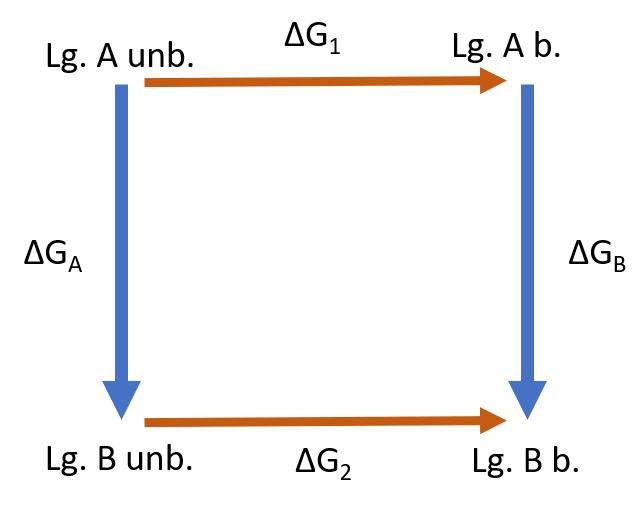
\includegraphics[scale=0.8]{cycle1}\caption{Thermodynamic cycle; red arrows indicate transitions between two states
(unbound--bound) of each ligand, blue arrows indicate 'alchemical'
transformations (Ligand~A--Ligand~B)\label{fig:cycle}}

\end{figure}

In general, the free energy is given by $F=-k_{B}T\ln Q$, where Q denotes the partition function $Q=\int dr\exp\left(-\beta U\right)$
with $\beta=\frac{1}{k_{B}T}$. Hence, the free energy difference between
states i and j can be described as \cite{Shirts.2013}:

\begin{equation}
\bigtriangleup F_{ij}=-\frac{1}{\beta}\ln\frac{Z_{j}}{Z_{i}}.
\end{equation}

To compute the free energy differences between two states, various
methods exist. Usually, it is not possible to simply compute the difference
between the two end states; hence, intermediate states have to be taken
into account. The difference between the final states can be expressed
as the sum of the difference between these intermediate states: $\Delta F=F_{1}-F_{0}=\sum_{n}\Delta F_{n}$
\cite{Mey.2020}.

\section{Methods for evaluating free energy differences}

Various approaches for calculating free energy differences exist,
e.g., thermodynamic integration and perturbation. Implementations of the latter approach use
the Zwanzig formula or Bennett's acceptance ratio method (which is
used in the {\trafo} package described below). In the following,
these three approaches will be briefly outlined. (For a more
comprehensive comparison and estimation of performance differences,
see \cite{Bruckner.2011} and \cite{Ruiter.2013}).

\subsection{Thermodynamic Integration (TI)}

In Thermodynamic Integration\cite{Kirkwood.1935}, the free energy difference between two
states is computed by evaluating the integral over the derivative of the free energy
between the initial and the final state of the transformation/process studied. TI computes intermediate
states depending on the coupling parameter $\lambda$. $\lambda=0$
and $\lambda=1$ represent the physical, initial / final states of
the system. Scaling between those two values, i.e., using values $0\le\lambda\le1$,
gives rise to the nonphysical, 'alchemical' intermediate states.

Taking the derivative of the free energy, one gets $\frac{dF}{d\lambda}=\frac{d}{d\lambda}\int e^{-\beta U dr}=\left\langle \frac{dU\left(r,\lambda\right)}{d\lambda}\right\rangle _{\lambda}$\cite{Shirts.2013}, 
where the angular brackets indicate the ensemble average.
The free energy difference is then given as the integral from $\lambda=0$ to $\lambda=1$:
\begin{equation}
\Delta F=
\intop_{\lambda=0}^{\lambda=1}\frac{dF\left(\lambda\right)}{d\lambda}d\lambda=
\intop_{\lambda=0}^{\lambda=1}\left\langle\frac{\partial U\left(\lambda\right)}{\partial\lambda}\right\rangle_\lambda d\lambda
.
\end{equation}
\begin{sloppypar}This integral has to be approximated using numerical integration, i.e., $\Delta F\approx\sum_{i}w_{i}\left\langle \frac{dU\left(r,\lambda\right)}{d\lambda}\right\rangle _{\lambda_{i}}$.
The weights $w_{i}$ depend on the choice of the numerical quadrature scheme.
A popular and simple choice is the trapezoidal rule, which in its most basic form uses equal
spacing between states and approximates the integral by $\intop_{\lambda=j}^{\lambda=i}\frac{dF\left(\lambda\right)}{d\lambda}d\lambda\approx\frac{i-j}{2}\left(f_{i}+f_{j}\right)$.
More efficient schemes can lower the number of necessary ${\lambda}$-states, e.g., Simpson's rule, Gauss-Legendre Quadrature, cubic spline interpolation  or Clenshaw-Curtis integration. Furthermore, usage of non-equidistant spacing, which can be easily be applied for the trapezoidal rule, but also for Simpson's rule, can improve efficiency.
For alchemical free energy simulations, it seems advisable to include the endpoints since those are the only physical states of the simulations (e.g., in Gauss-Legendre quadrature the endpoints are not included). \cite{Bruckner.2011, Bruckner.2011b} \end{sloppypar}

In any case, the integration scheme and the amount of intermediate steps has to
be chosen in such a way that the introduced bias is below the statistical
noise\cite{Shirts.2013}. (For a more detailed comparison of various numerical quadrature
schemes, e.g., the trapezoidal rule and Simpson's rule, see \cite{Bruckner.2011b}). 

\subsection{Free Energy Perturbation / Zwanzig Relation}

Free energy perturbation relies on the Zwanzig relation (sometimes called exponential
formula). For each configuration of state A, the energy difference
between this state and the corresponding state B is calculated, which is then used to compute the free energy difference between A and B according to \cite{Zwanzig.1954,Gapsys.2015}
\begin{equation}
\Delta F_{A\rightarrow B}=F_{B}-F_{A}=-\frac{1}{\beta}\ln\frac{Q_{B}}{Q_{A}}=-k_{b}T\ln\left\langle \exp\left(\frac{-\Delta U_{A\rightarrow B}}{k_{B}T}\right)\right\rangle _{A}.
\end{equation}

Several variants of the formula exist: For instance, one can either
calculate forward or backward perturbations (either $\Delta F\left(A\rightarrow B\right)$ or
$-\Delta F\left(B\rightarrow A\right)$), or, as it is
usually the case, use double-wide sampling where energy differences
from both directions are processed \cite{Bruckner.2011}.

As for thermodynamic integration, usually it is necessary to
introduce intermediate states. The free energy between the final states
0 and 1 is calculated as the sum of the differences between all adjacent
intermediate states; in the case of n states: $\Delta F_{0\rightarrow1}=\sum_{i=0}^{n-1}\left(F\left(i+1\right)-F\left(i\right)\right)$.
There has to be a sufficient number of intermediate states --- there must be significant overlap between the two states --- otherwise convergence is poor.
However, there are still use cases when other methods are not feasible\cite{Boresch.2017},
and there exists an extension to non-equilibrium work (Jarzynski's
equation)\cite{Boresch.2017}. In general, however, it should be only used
if the difference between the two states are tiny\cite{Shirts.2013}.

\subsection{Bennett Acceptance Ratio (BAR)}

An extension of the perturbation approach for computing the free energy difference between
two states is Bennett's Acceptance Ratio\cite{Bennett.1976}. 

Expansion of the denominator and numerator of the ratio of the canonical
partition functions of both states leads to: 
\begin{equation}
\frac{Q_{0}}{Q_{1}}=\frac{Q_{0}\int W\exp\left(-U_{0}-U_{1}\right)dq^{N}}{Q_{1}\int W\exp\left(-U_{0}-U_{1}\right)dq^{N}}=\frac{\left\langle W\exp\left(-U_{0}\right)\right\rangle _{1}}{\left\langle W\exp\left(-U_{1}\right)\right\rangle _{0}}
\end{equation}
where W denotes a (for now arbitrary) weighting function. Assuming
a Gaussian distribution of the estimation error in the limit of large
samples, the optimal W can be determined as $W\left(q_{1}...q_{n}\right)=c\left(\frac{Q_{0}}{n_{0}}\exp\left(-U_{1}\right)+\frac{Q_{1}}{n_{1}}\exp\left(-U_{0}\right)\right)^{-1}$\cite{Bennett.1976}. 

To use Bennett's acceptance ratio method, two simulations have
to be carried out. One starts at $\lambda=0$, the other one at $\lambda=1$.
Forward and backward simulations are processed simultaneously. 

The free energy difference between two $\lambda$-states can be expressed as
\begin{equation}
\bigtriangleup F\left(\lambda_{i}\rightarrow\lambda_{j}\right)=\beta^{-1}\left(\ln\frac{\left\langle f\left(U_{\lambda_{i}}-U_{\lambda_{j}}+C\right)\right\rangle _{\lambda_{j}}}{\left\langle f\left(U_{\lambda_{j}}-U_{\lambda_{i}}+C\right)\right\rangle _{\lambda_{i}}}\right)+C
\end{equation}
with the Fermi function $f\left(x\right)=\frac{1}{1+\exp\left(\beta x\right)}$
\cite{Bruckner.2011,Gapsys.2015}.

To obtain the value of the optimum shift constant,
\begin{equation}
C=\beta^{-1}\ln\frac{Q_{i}N_{j}}{Q_{j}N_{i}},
\end{equation}
a self-consistency
problem has to be solved iteratively\cite{Gapsys.2015}.

The free energy between two $\lambda$-states is then given by $\bigtriangleup F\left(\lambda_{i}\rightarrow\lambda_{j}\right)=\beta^{-1}\ln\frac{N_{j}}{N_{i}}+C$\cite{Bruckner.2011}.
$N_{j}$ and $N_{i}$denote the number of sampled configurations from
state j and i, respectively.

BAR gives a minimal variance free energy estimate. There is also an
alternative derivation for the formula. It can be shown that the
Bennett acceptance ratio method works as a maximum likelihood estimator.
Using BAR, one obtains the asymptotically unbiased estimation (i.e., for an infinite
number of measurements it yields an unbiased estimation) 
with the lowest variance\cite{Shirts.2003}. 

Using variational calculus to minimize the variance, $\Delta F$ can
be expressed implicitly as:$\frac{\partial\ln L\left(\Delta F\right)}{\partial\Delta F}=\sum\frac{1}{1+\exp\left(\beta\left(M+W_{i}-\Delta F\right)\right)}-\sum\frac{1}{1+\exp\left(\beta\left(M-W_{j}-\Delta F\right)\right)}=0$
, where M denotes $M=\beta^{-1}\ln\frac{N_{j}}{N_{i}}$ \cite{Shirts.2003}.

BAR also depends on the overlap between the states; however, it is
more robust and reliable in cases of rather poor overlap \cite{Ruiter.2013}
(especially when compared to FEP). In any case, phase space overlap is a necessary condition, without overlap the method will fail. (Whether BAR outperforms thermodynamic
integration crucially depends on the smoothness of the integrand.
For more pronounced changes in molecular properties between the computed
states, BAR seems to be superior\cite{Shirts.2013}.)

MBAR, which is used in the {\trafo} package to estimate the free energy differences, is a further improvement of the BAR method. BAR combines information of one forward and one backward simulation.
In contrast to BAR, MBAR does not only consider samples two states, but data from all states is used.
Weights have to be determined for all state combinations. Again, the emerging equations give rise to a self-consistency problem which can be solved, e.g., via iteration methods or a Newton-Raphson solver. For state i, an estimation of free energy can be computed as \begin{equation}F_{i}=-\beta^{-1}\ln\mathop{\sum}_{j=1}^{K}\sum_{n=1}^{N_{j}}\frac{\exp\left(-\beta u_{i}\right)}{\sum_{k=1}^{K}N_{k}\left(\beta F_{k}-\beta u_{k}\right)}\end{equation}. 
The estimate depends on all samples K, in the case of only two states, MBAR reduces to BAR. Although this formula gives the estimation for state i, it is determined only up to an additive constant. Thus, only energy differences, \bigtriangleup $F_{ij}=F_{j}-F_{i}$ are meaningful. \cite{Shirts.2008} 
MBAR is also related to another technique for evaluating free energy differences, the weighted histogram analysis method (WHAM)\cite{Kumar.1992}. As in MBAR, data from all samples is used simultaneously, but the data is partitioned into bins which are used to generate histograms of the probabilities. Here MBAR equals the limiting case for a bin width of zero.\cite{Shirts.2008, Klimovich.2015} 

\section{Soft-core potentials}

Alchemical transformations rely on a coupling parameter $\lambda$ which
is used to gradually modify interactions. For example, by scaling $\lambda$, one can weaken the interaction with one part of the system and remove them completely at the final state. (In the simplest case,
there are only two states corresponding, e.g., to an atom present in
one of the two molecules but not in the other one. If the two molecules
have more considerable differences, this annihilation process has to be carried out for each atom, which has to be transformed
into a dummy atom.)
The term 'van der Waals endpoint problem' (or even 'catastrophe') denotes
several problems which can occur when a particle is removed (i.e.,
turned into a dummy atom by turning off its intermolecular interactions).
\cite{Boresch.2011}

We illustrate the types of problems, which can arise, for the case
of a linear dependence of the coupling parameter,
i.e.

\begin{equation}
U\left(\lambda\right)=U_{o}+\lambda\sum_{1\leq i\leq N-1}u_{i,N}.
\end{equation}


(Of course, the equal spacing of the coupling parameter does not imply
equal phase-space overlap between the states \cite{Shirts.2013};
thus, for many simulations this simple set-up is certainly not the
optimal solution.) For $\lambda=0$ and $\lambda\approx0$ various
issues emerge. If $\lambda=0$, there are no interactions (and hence
no repulsion) and the non-interacting dummy particle can be located
at the exact position of another particle. This could give rise to
errors resulting from divisions by zero. (In contrast to the next two scenarios,
this seems to be a minor problem avoidable by efficient coding, i.e.,
implementing an additional clause for this condition to avoid the division by zero. In fact, it appears that all common MD
simulations packages manage this case automatically\cite{Boresch.2011}).

For $\lambda\rightarrow0$, numerical instabilities can occur because
even within a small time-step the interactions can become highly repulsive.
It should be noted that this problem emerges at values $\lambda\approx0$,
but not at $\lambda=0$ (i.e., when the particles are completely decoupled).

If thermodynamic integration is used, a related problem occurs because
$\left\langle \frac{\partial U}{\partial\lambda}\right\rangle _{\lambda}$can
become singular. This is obvious for the example using a linear pathway:
$\frac{\partial U\left(\lambda\right)}{\partial\lambda}=\sum_{1\leq i\leq N-1}u_{i,N}$.
As for the problem leading to a division by zero, the fact that one of the
still interacting particles can be located at the same place
in the simulation box as the dummy atom causes this quantity to change
unpredictably and, in the worst case, become singular \cite{Boresch.2011}.

The established way to avoid such problems is the usage of soft-core potentials \cite{Beutler.1994,Zacharias.1994,Steinbrecher.2011}.
An additional term is added to the particle-particle distance in the Lennard-Jones potential so that
no division by 0 occurs and the corresponding derivative does not
become singular. One possibility is that the usual Lennard-Jones potential is replaced by
a slightly modified potential which ensures that at $r=0,\lambda>\text{0}$
the divisor is never 0 and the division by zero is avoided:

\begin{equation}
U_{LJ}\left(r,\lambda\right)=\left(1-\lambda\right)\left(\frac{A}{\left(r^{2}+\lambda\delta\right)^{6}}-\frac{B}{\left(r^{2}+\lambda\delta\right)^{3}}\right)
\end{equation}

However, the usage of soft-core potentials has some limitations. In
particular, the availability of soft-core potentials depends on the
used software package. Free energy calculations have to be explicitly
supported. 

\section{Dummy atoms, Single/Dual topology}

Usually, the number of atoms of both molecules of interest, i.e., of the
two end states of an alchemical free energy calculation, is not
the same. However, the atom number has to stay constant (as the simulation
takes place in the canonical ensemble). Because of that constraint,
so-called dummy atoms are necessary \cite{Fleck.2021}. These dummy
atoms do not participate in any non-bonded interactions, but they
have to be connected via bonded interactions to the rest of the molecule
they belong to so that they do not get detached and float through
the simulation box.

There are two main approaches for setting up alchemical mutations, both involving dummy atoms: 

In single topology, during the mutation process, physical atoms, which belong only to the start state, are
transformed into dummy atoms at the end state. Conversely, 
as the alchemical transformation proceeds, dummy atoms present at the initial state are re-transformed
into physical atoms of the second molecule.

In dual topology, no direct mutation of real atoms into dummy atoms
occurs. However, both physical molecules are augmented with all dummy
atoms of the respective other state (hence, there is no state during the simulation
without dummy atoms). Thus, the number of dummy atoms equals the number
of atoms which have no direct correspondence in the other molecule.
Usually, in total, even more dummy atoms are present in the system
as in a single topology setup \cite{Fleck.2021}.

The implementation of such dummy atoms, however, is not without pitfalls.
In single topology, errors can arise if too many bonded interactions are kept. The order in which interactions are turned off has to be constrained
by specific rules to ensure that the contributions exactly cancel
out each other, and attention has to be paid to under which conditions
dummy atom contributions cancel out exactly. \cite{Fleck.2021}

\section{Serial atom insertion}

As an alternative to modifying the coupling parameter, one can
try to create new states by turning off atoms in one step without
intermediate values. This approach, called serial atom insertion, was introduced In \cite{Boresch.2011}. Atoms are turned off serially (one after one
or in small batches). There is no gradual damping of the interactions; the
LJ-interactions of a molecule are either present ($\lambda=1$) or
turned off ($\lambda=0$).

A sufficient phase space overlap between neighboring states is crucial
for any alchemical free energy calculation. So, the question arises
whether turning off one atom in one step is in agreement with this prerequisite. The feasibility of this approach relies on Bennett's acceptance
ratio, which was shown to work with neighboring states created
by serial atomic insertion \cite{Boresch.2011}.

In particular, serial atom insertion has the advantage that it works
even for MD programs which lack explicit support for free energy
simulations and soft-core potentials are not needed (because the coupling
parameter takes only the values 0 and 1). The free energy differences
between states can be assembled from 'normal' simulations.

The most severe restriction due to the van der Waals endpoint
problem is the instability of the integrator near the end state where an atom has almost vanished (i.e.,  $\lambda=0$ or  $\lambda=1$). As such states
are not used in serial atom insertion, this problem is automatically
avoided.

The feasibility of this approach depends on the sufficient overlap
between the states. Using BAR/MBAR, no intermediate steps are necessary
and atoms can be turned off one by one. Contrariwise, thermodynamic
integration cannot be used because it is precisely the scaling of the
interaction parameter between 0 and 1 which is avoided. This also
implies that the singularity risk of the derivative due to the van
der Waals endpoint problem can be neglected (as this part of the problem
only concerns thermodynamic integration).